\documentclass{article}
\usepackage[backend=biber,citestyle=ieee]{biblatex}
\usepackage[english]{babel}
% \usepackage[swedish]{babel}
\usepackage{graphicx}
\usepackage{csquotes}
\usepackage{float}
\usepackage{datetime}
\usepackage[title]{appendix}
\usepackage{subfig}
% \usepackage{a4wide} %For wider content on page
\usepackage{amsmath} %For multiline equations 
\usepackage{fancyhdr}   %page header
\pagestyle{fancy}

% \usepackage[parfill]{parskip} %Line skip between paragraphs instead of indent

\usepackage{xcolor}
\usepackage{listings}

\definecolor{codegreen}{rgb}{0,0.6,0}
\definecolor{codegray}{rgb}{0.5,0.5,0.5}
\definecolor{codepurple}{rgb}{0.58,0,0.82}
\definecolor{backcolour}{rgb}{0.95,0.95,0.95}
\lstdefinestyle{mystyle}{
    backgroundcolor=\color{backcolour},   
    commentstyle=\color{codegreen},
    keywordstyle=\color{magenta},
    numberstyle=\tiny\color{codegray},
    stringstyle=\color{codepurple},
    basicstyle=\ttfamily\footnotesize,
    breakatwhitespace=false,         
    breaklines=true,                 
    captionpos=b,                    
    keepspaces=false,                 
    numbers=left,                    
    numbersep=5pt,                  
    showspaces=false,                
    showstringspaces=false,
    showtabs=false,                  
    tabsize=1
}
\lstset{style=mystyle}


\addbibresource{sources.bib}

\newcommand{\getauthor}{Elias Berglin} %Author
\newcommand{\gettitle}{Labb2} %Title

\newdateformat{daymonthyear}{\ordinal{DAY} \monthname[\THEMONTH] \THEYEAR} %Date

\title{\gettitle}
\author{\getauthor}

\date{\daymonthyear\today} %Remove for swedish date

\begin{document}

    % Title 
    \pagenumbering{gobble}
    \maketitle
    \newpage

    % Page header and footer
    \pagenumbering{arabic}
    \fancyhf{}
    \lhead{\getauthor}
    \rhead{\gettitle}
    \rfoot \thepage

    % Document starts here
    \section{Week 3}
    \subsection{Assignment}
    \subsubsection{Hough transform}
    The code I used to transform and draw the graphs can be found in appendix \ref{appendix:hough}. 
    Figure \ref{fig:ha} shows task a/b and figure \ref{fig:hc} shows task c.
    \begin{figure}[H]
        \centering
        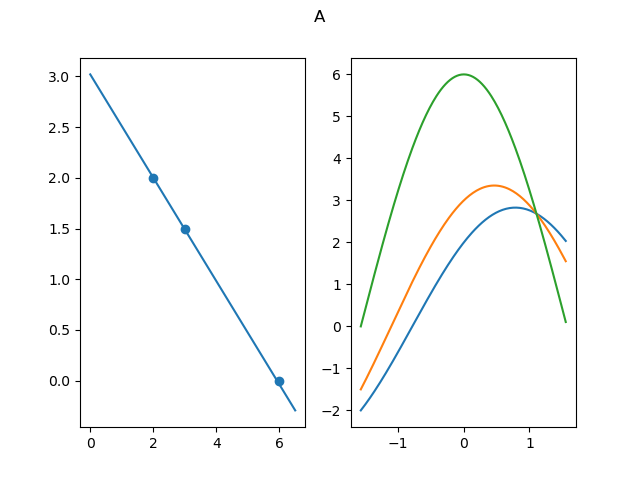
\includegraphics[width=1\textwidth]{Finished/HoughA.png}
        \caption{Task a/b. Image space on the left and hough space on right}
        \label{fig:ha}
    \end{figure}
    \begin{figure}[H]
        \centering
        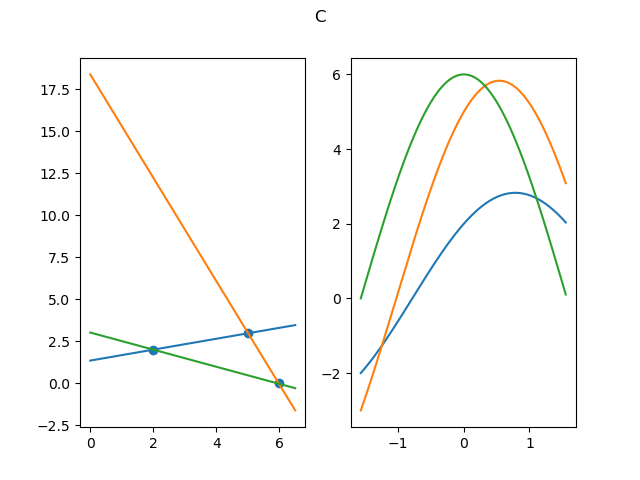
\includegraphics[width=1\textwidth]{Finished/HoughB.png}
        \caption{Task c. Image space on the left and hough space on right}
        \label{fig:hc}
    \end{figure}
    \subsubsection{Feature descriptors}
    I have read 2 comparison papers between different feature descriptors. SIFT seems to always be the most acurate.
    But it is also not as fast. Considoring we have an AR application we need to have a somewhat faster algorithm
    to make it easier to track features. These papers say that ORB is almost as good as SIFT but much faster so I would
    go with ORB for my AR application. \cite{art1} \cite{tareen2018comparative}
    \subsubsection{Feature detection (and matching)}
    Python code used for the assignment can be found in appendix \ref{appendix:code}.
    Figure \ref{fig:img1} shows the features extracted from the first images using SIFT and my Harris implementation. Figure \ref{fig:img2}
    shows the features extracted from the second image using SIFT and my Harris implementation.

    \begin{figure}[H]
        \centering
        \subfloat{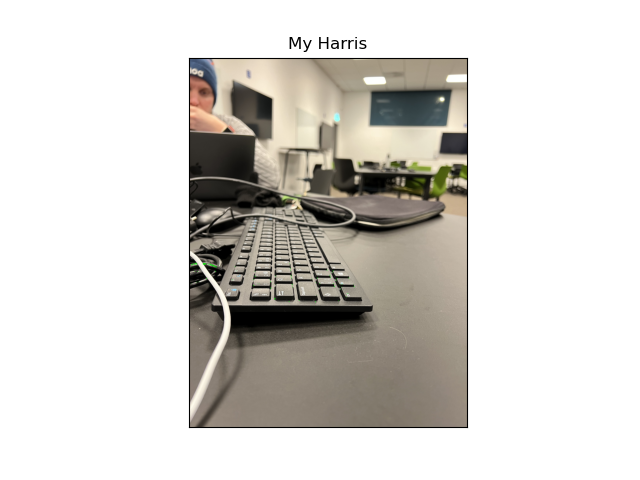
\includegraphics[width=8cm]{Finished/Start1_My_Harris_detector.png}}
        \quad
        \subfloat{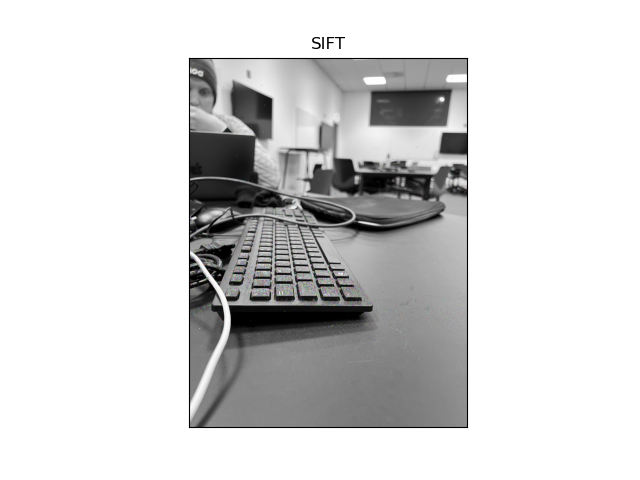
\includegraphics[width=8cm]{Finished/Start1_SIFT_Detector.png}}
        \caption{First image with Harris and SIFT}
        \label{fig:img1}
    \end{figure}
    \begin{figure}[H]
        \centering
        \subfloat{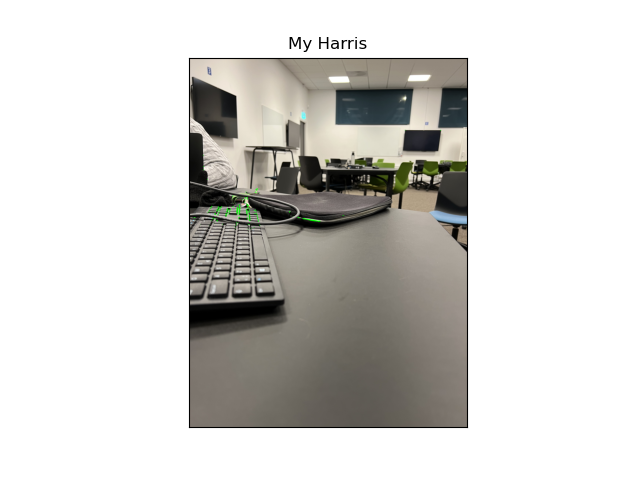
\includegraphics[width=8cm]{Finished/Start2_My_Harris_detector.png}}
        \quad
        \subfloat{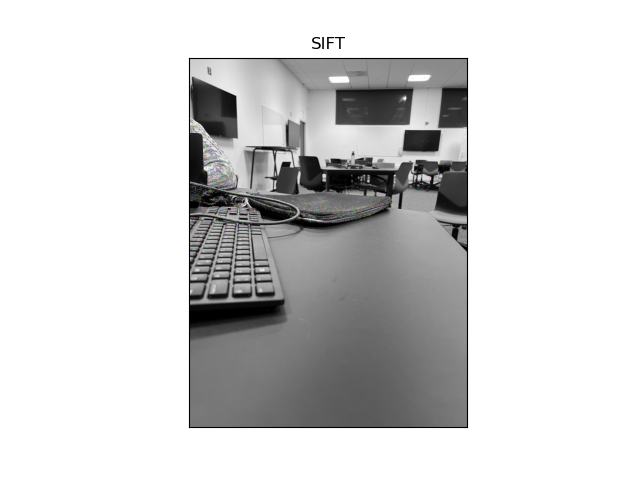
\includegraphics[width=8cm]{Finished/Start2_SIFT_Detector.png}}
        \caption{Second image with Harris and SIFT}
        \label{fig:img2}
    \end{figure}
    \subsection{Reflection}
    This week was interesting. 
    I thought that feature detection/descriptors was a really interesting subject.
    The most interesting part was reading the research papers where they benchmarked
    different algorithms for finding features. I had a hard time grasping the concept
    of Hough transform but after watching the YouTube course I quickly understood
    how it worked. This has been the fact for all of the weeks. If I don't fully
    understand something during the lecture the YouTube course have always cleard
    it up for me.

    My Harris detector did not performe well compared to SIFT. But when I compared it
    to the OpenCV implementation it was not far off. From reading the papers \cite{art1} \cite{tareen2018comparative}
    I now understand that SIFT is really good at finding features and thus it is understandable that
    Harris does not perform ass well


    \section{Week 4}
    \subsection{Assingment}
    \subsubsection{2D Transformations}
    The question was for a similarity transform but we are not doing any scaling so we are
    really doing an euclidian transformation so the folling matrix was created based
    on the lecture slides:
    \begin{equation}
        \begin{pmatrix}
            cos(15*\frac{\pi}{180}) & -sin(15*\frac{\pi}{180}) & 3 \\
            sin(15*\frac{\pi}{180}) & cos(15*\frac{\pi}{180}) & -2 \\
            0 & 0 & 1 \\
            \end{pmatrix}
    \end{equation}

    To calculate the transfomration matrix (homography matrix) the code in appendix \ref{appendix:homo} was used
    and the following matrix was calculated:
    \begin{equation}
        \begin{pmatrix}
            1.8  & 0.67 & 1 \\
            0.6 & 0.67 & 1\\
            0.2 & 0 & 1 \\
            \end{pmatrix}
    \end{equation}
    
    \subsubsection{Stereo estimation}
    I had ha hard time understanding the website interface so I just took the first
    algorithm with a paper connected to it. So I chose RAFT-Sterio \cite{lipson2021raft}.
    This algorithm is based on RAFT \cite{teed2020raft} and extends the concepts of GRU
    \subsubsection{Plane Sweep}
    Full code for Plane Sweep algorithm can be found in \ref{appendix:PS}. The images used as input can be found in figure \ref{fig:psOrigi},
    the depth image can be found in figure \ref{fig:ps}.
    \begin{figure}[H]
        \centering
        \subfloat{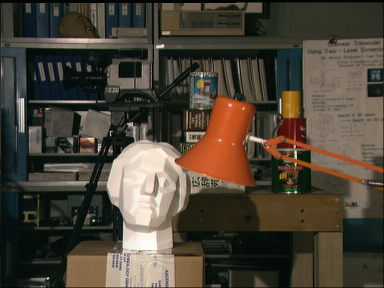
\includegraphics[width=5cm]{ps1.png}}
        \quad
        \subfloat{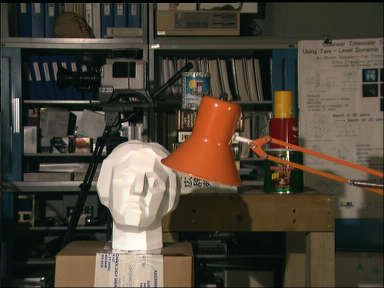
\includegraphics[width=5cm]{ps2.png}}
        \caption{Imaged used to for Plane Sweep algorithm}
        \label{fig:psOrigi}
    \end{figure}
    \begin{figure}[H]
        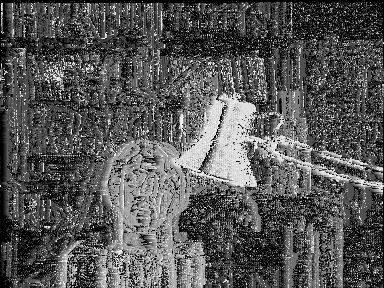
\includegraphics[width=1\textwidth]{sd.png}
        \caption{Images produced from Plane Sweep algorithm}
        \label{fig:ps}
    \end{figure}
    \subsubsection{Stitching}
    The code used to stitch images can be found in appendix \ref{appendix:IS}
    My own implementation of RANSAC and calculation of the homography matrix was used. To find feature points
    ORB was used, implemented by OpenCV. To match feature points a Brute Force Matcher from OpenCV was used. This was then used in KNN to get K best matches
    for each point. I then use a perspective warp to warp one image and then apply the other image on top of that image. 
    The images used for stitching can be found in figure \ref{fig:originalStitch} and the produced output can be found in figure \ref{fig:stiched}.

    \begin{figure}[H]
        \centering
        \subfloat{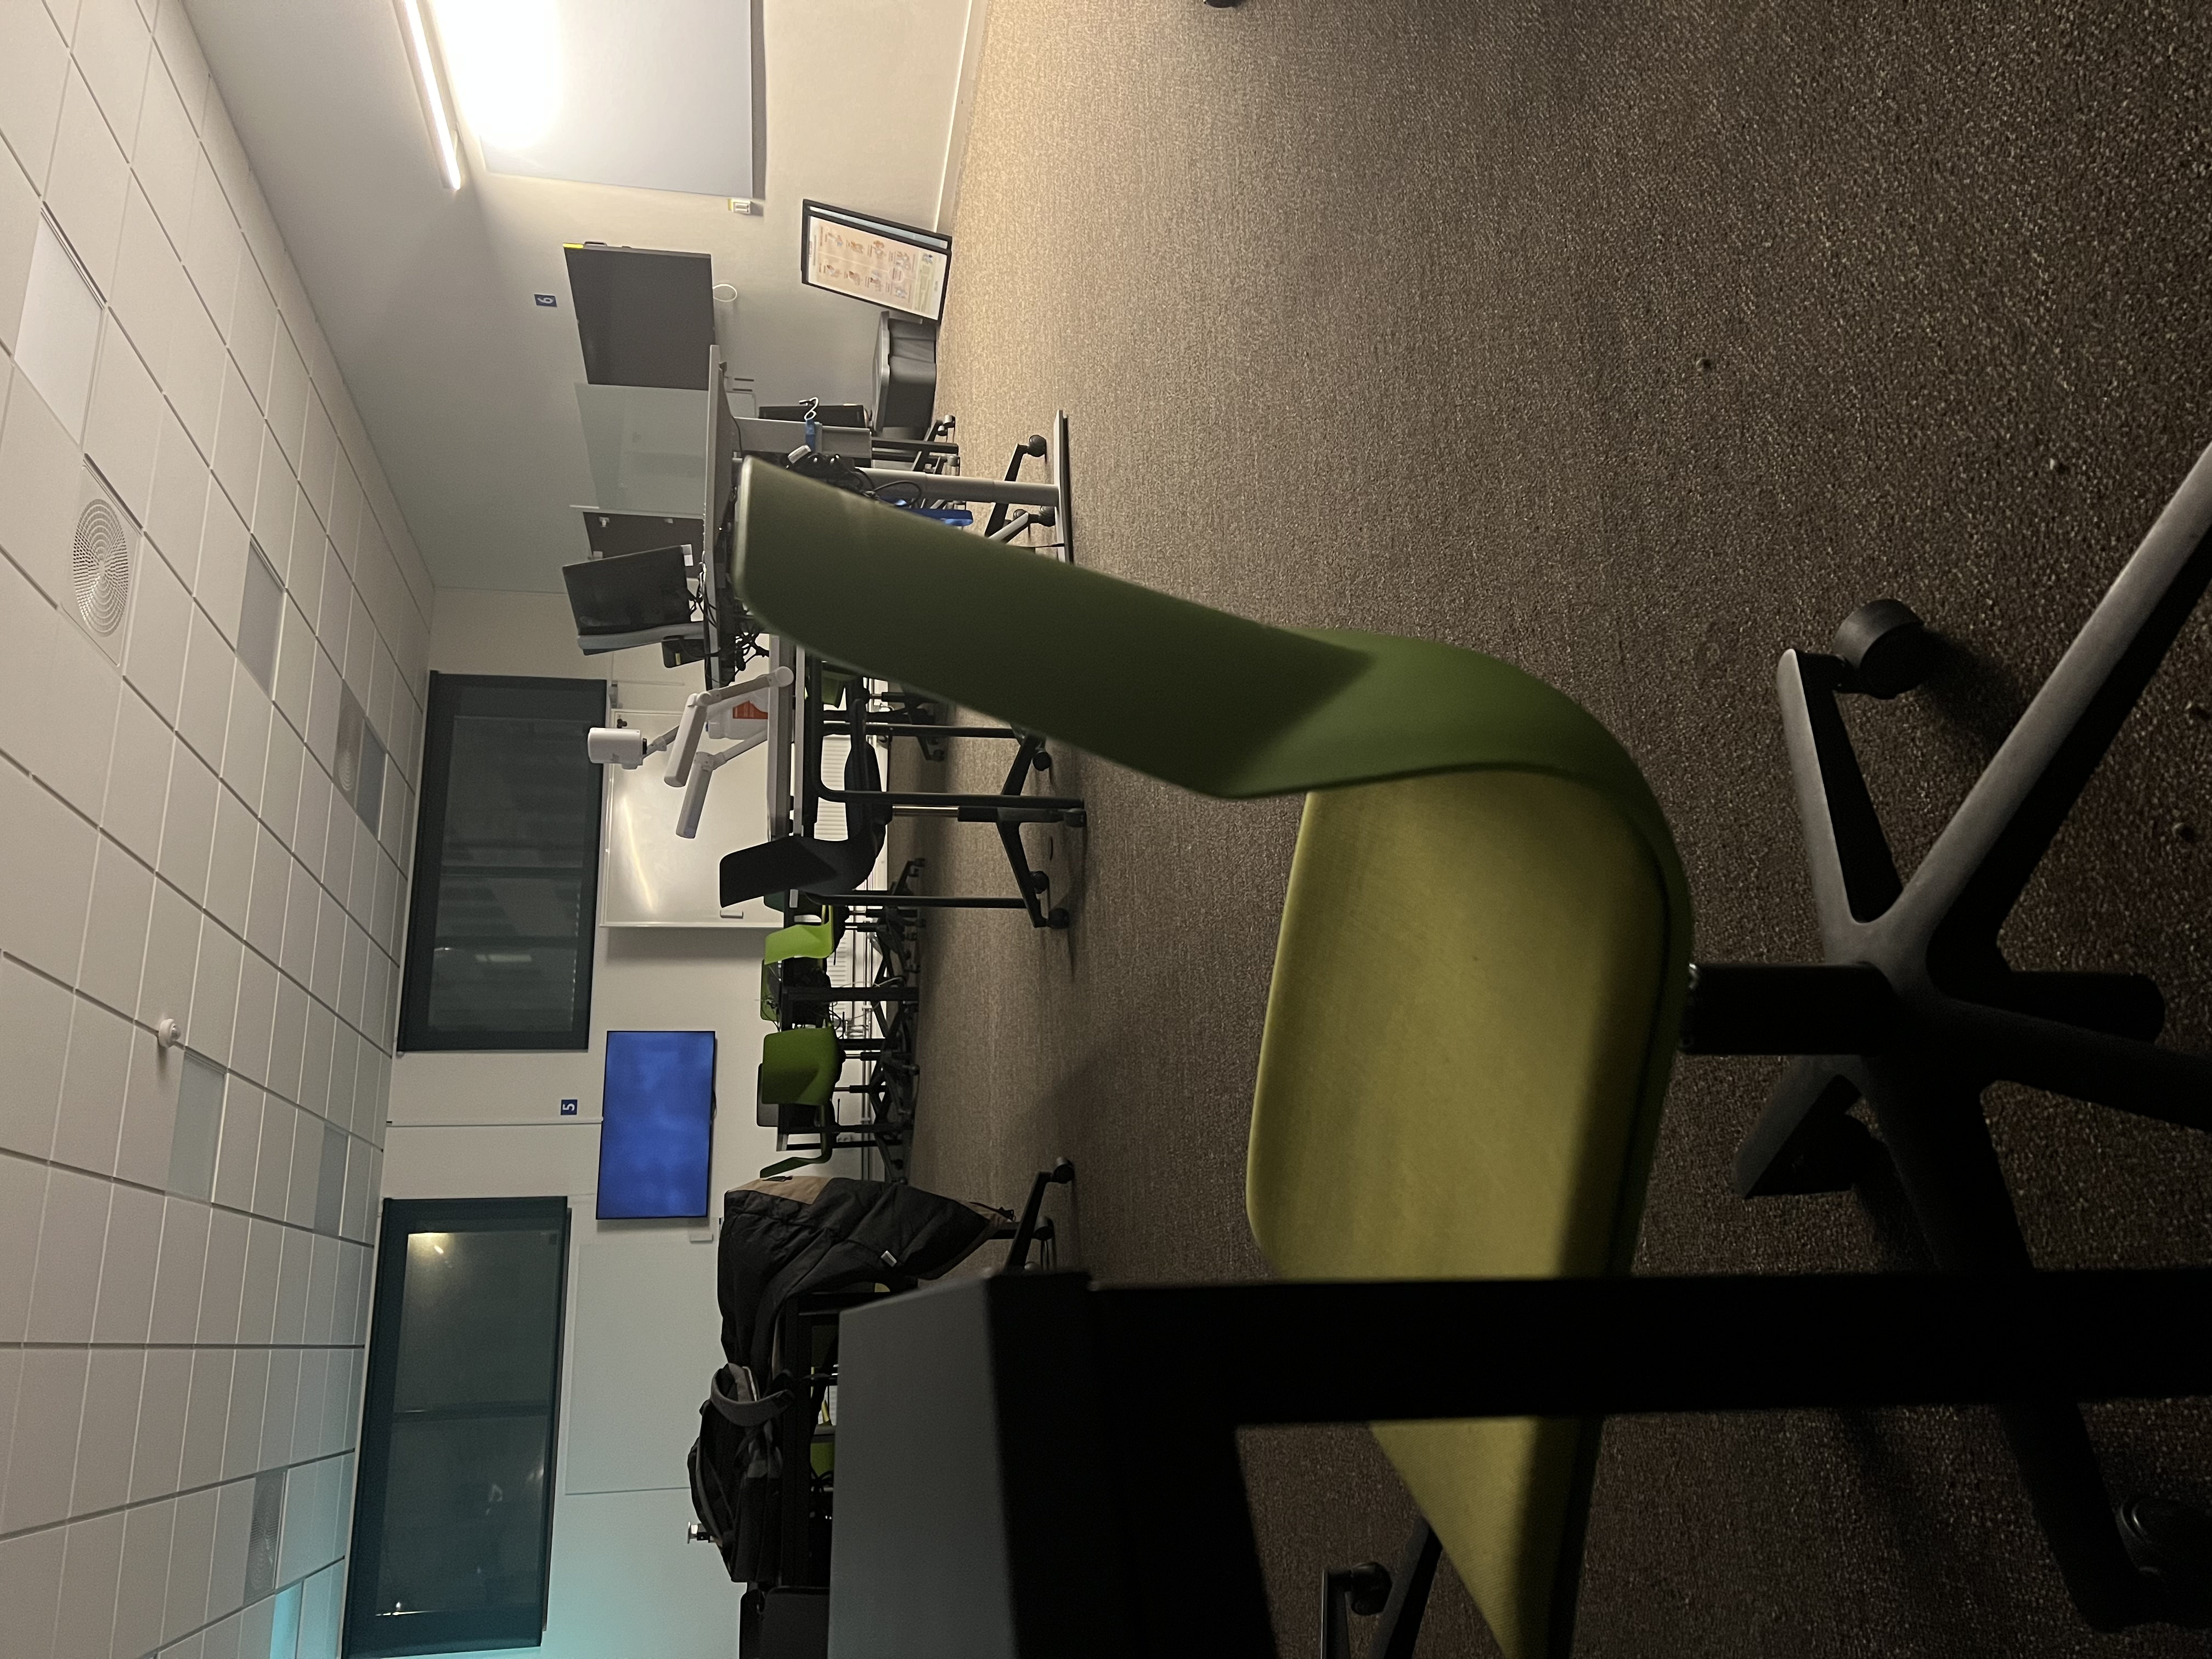
\includegraphics[width=5cm]{right.jpg}}
        \quad
        \subfloat{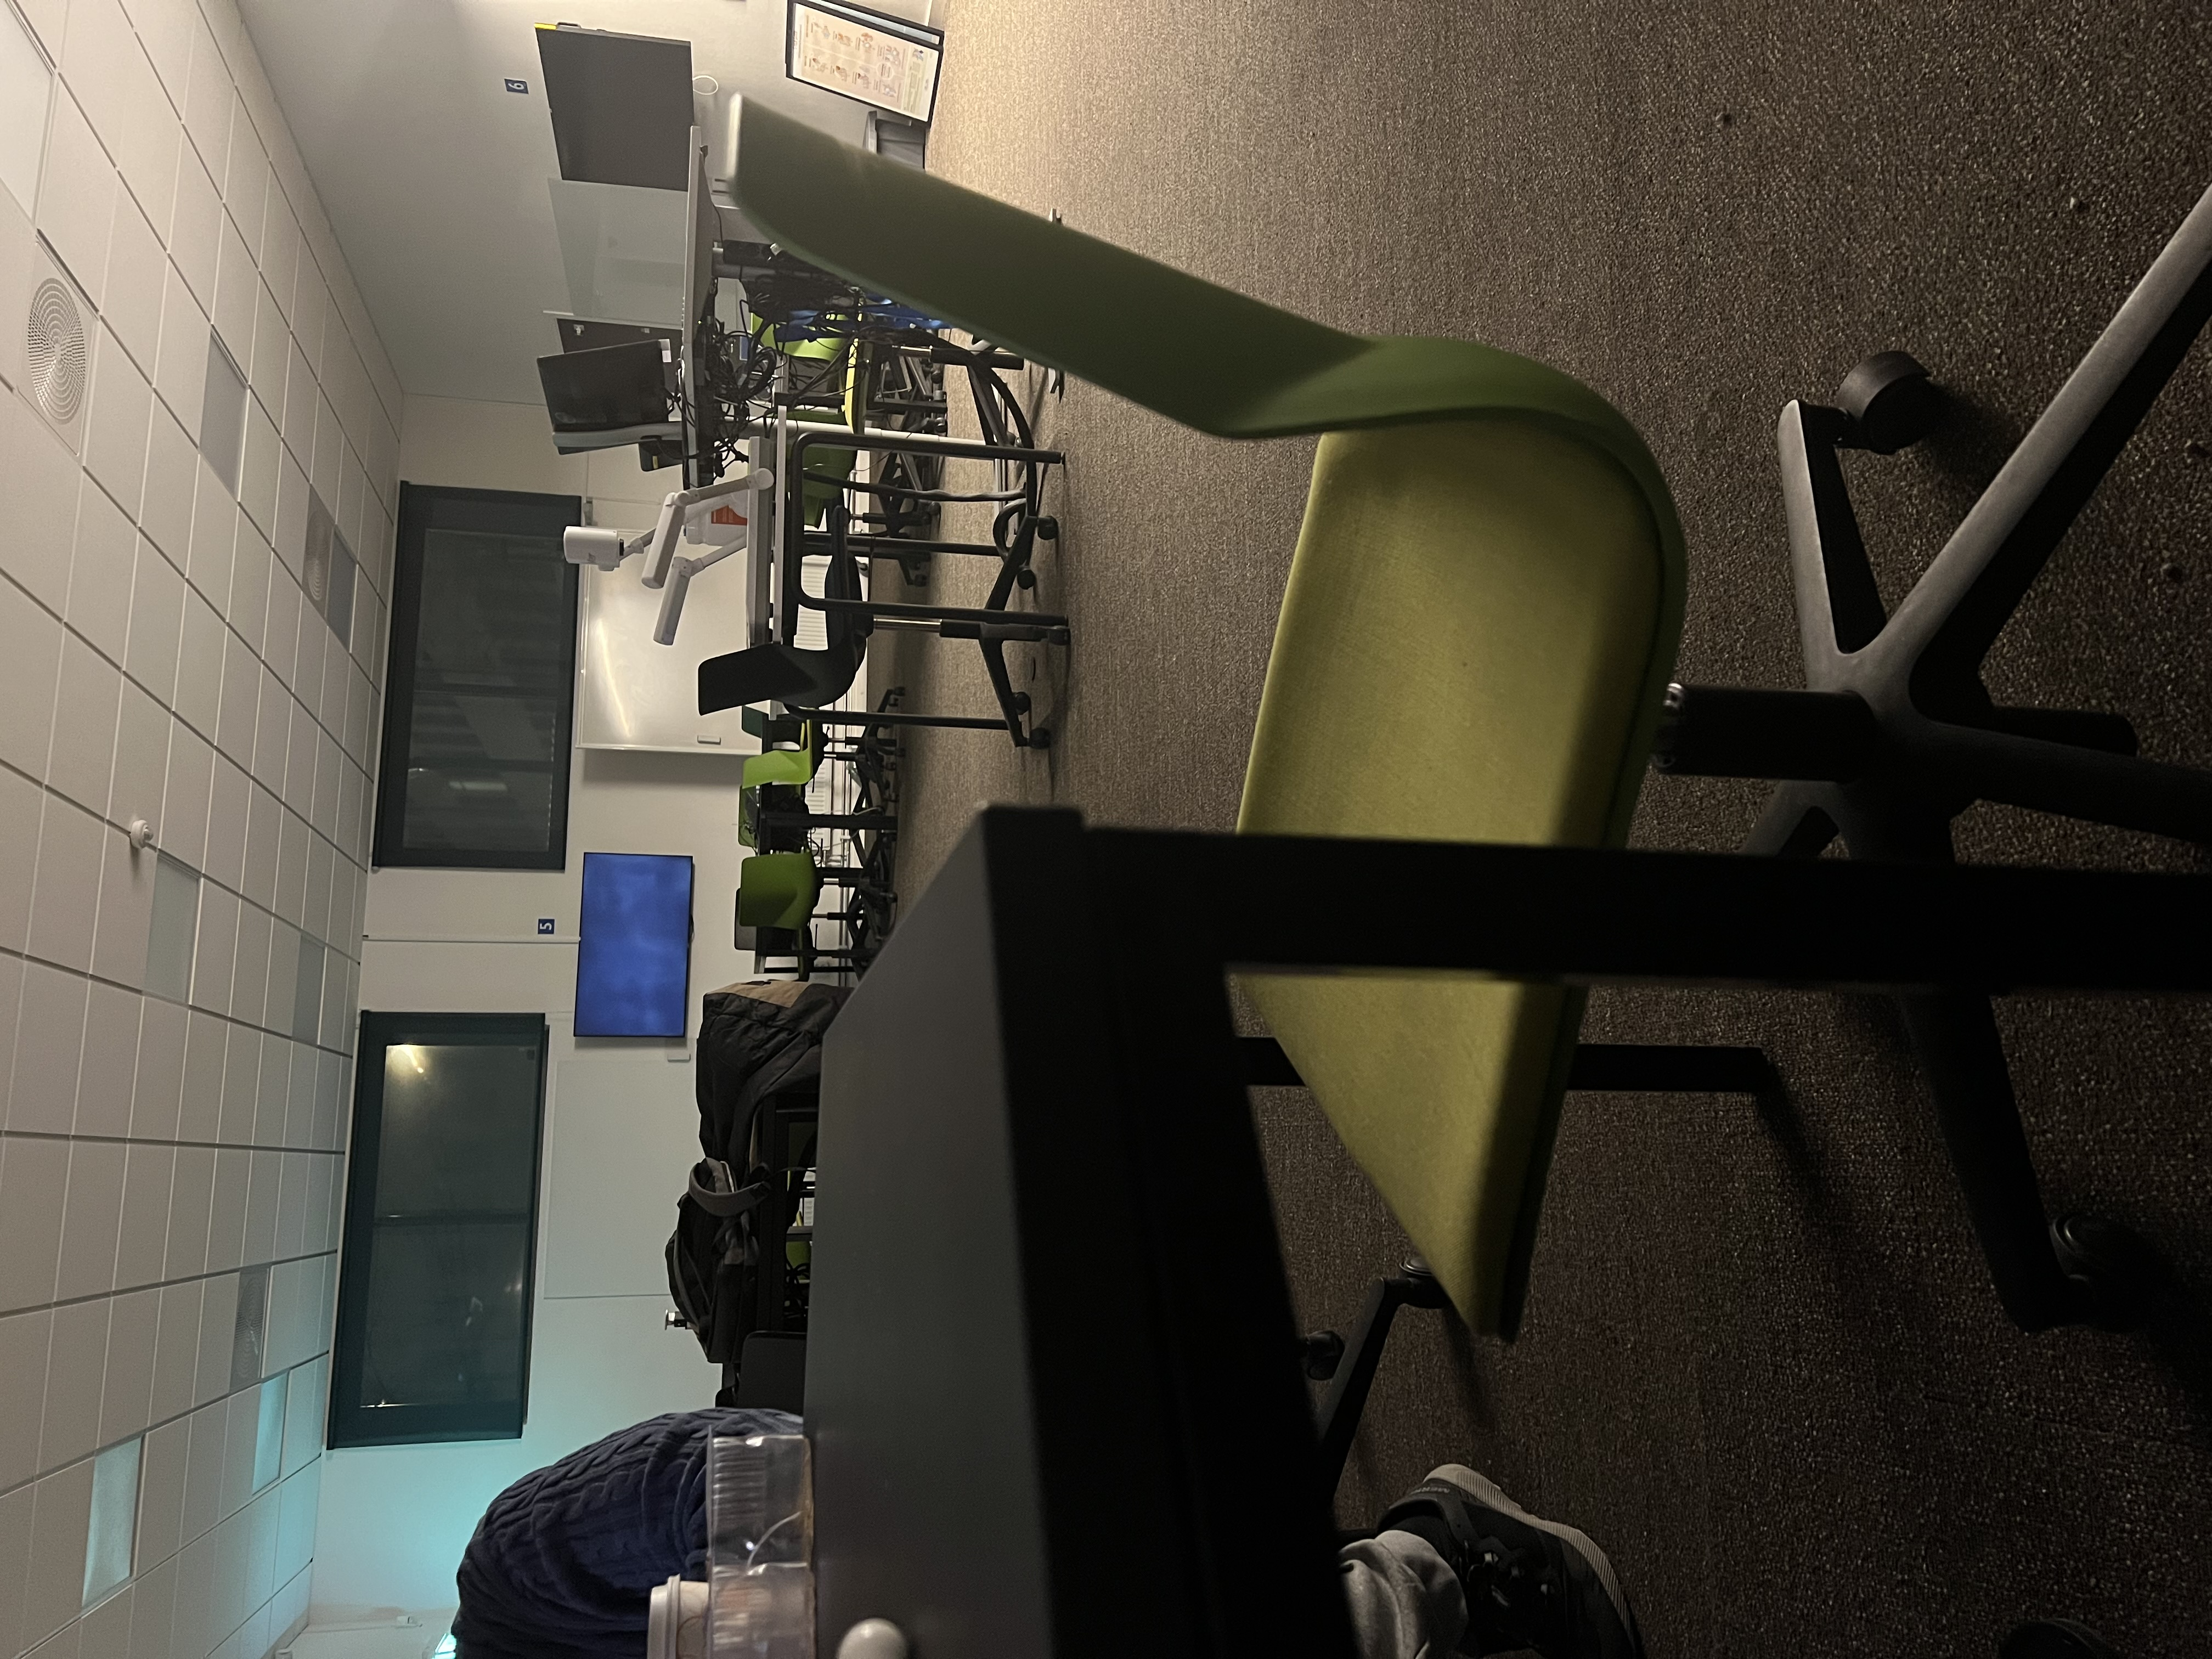
\includegraphics[width=5cm]{left.jpg}}
        \caption{Images used for Stitching}
        \label{fig:originalStitch}
    \end{figure}
    \begin{figure}[H]
        \centering
        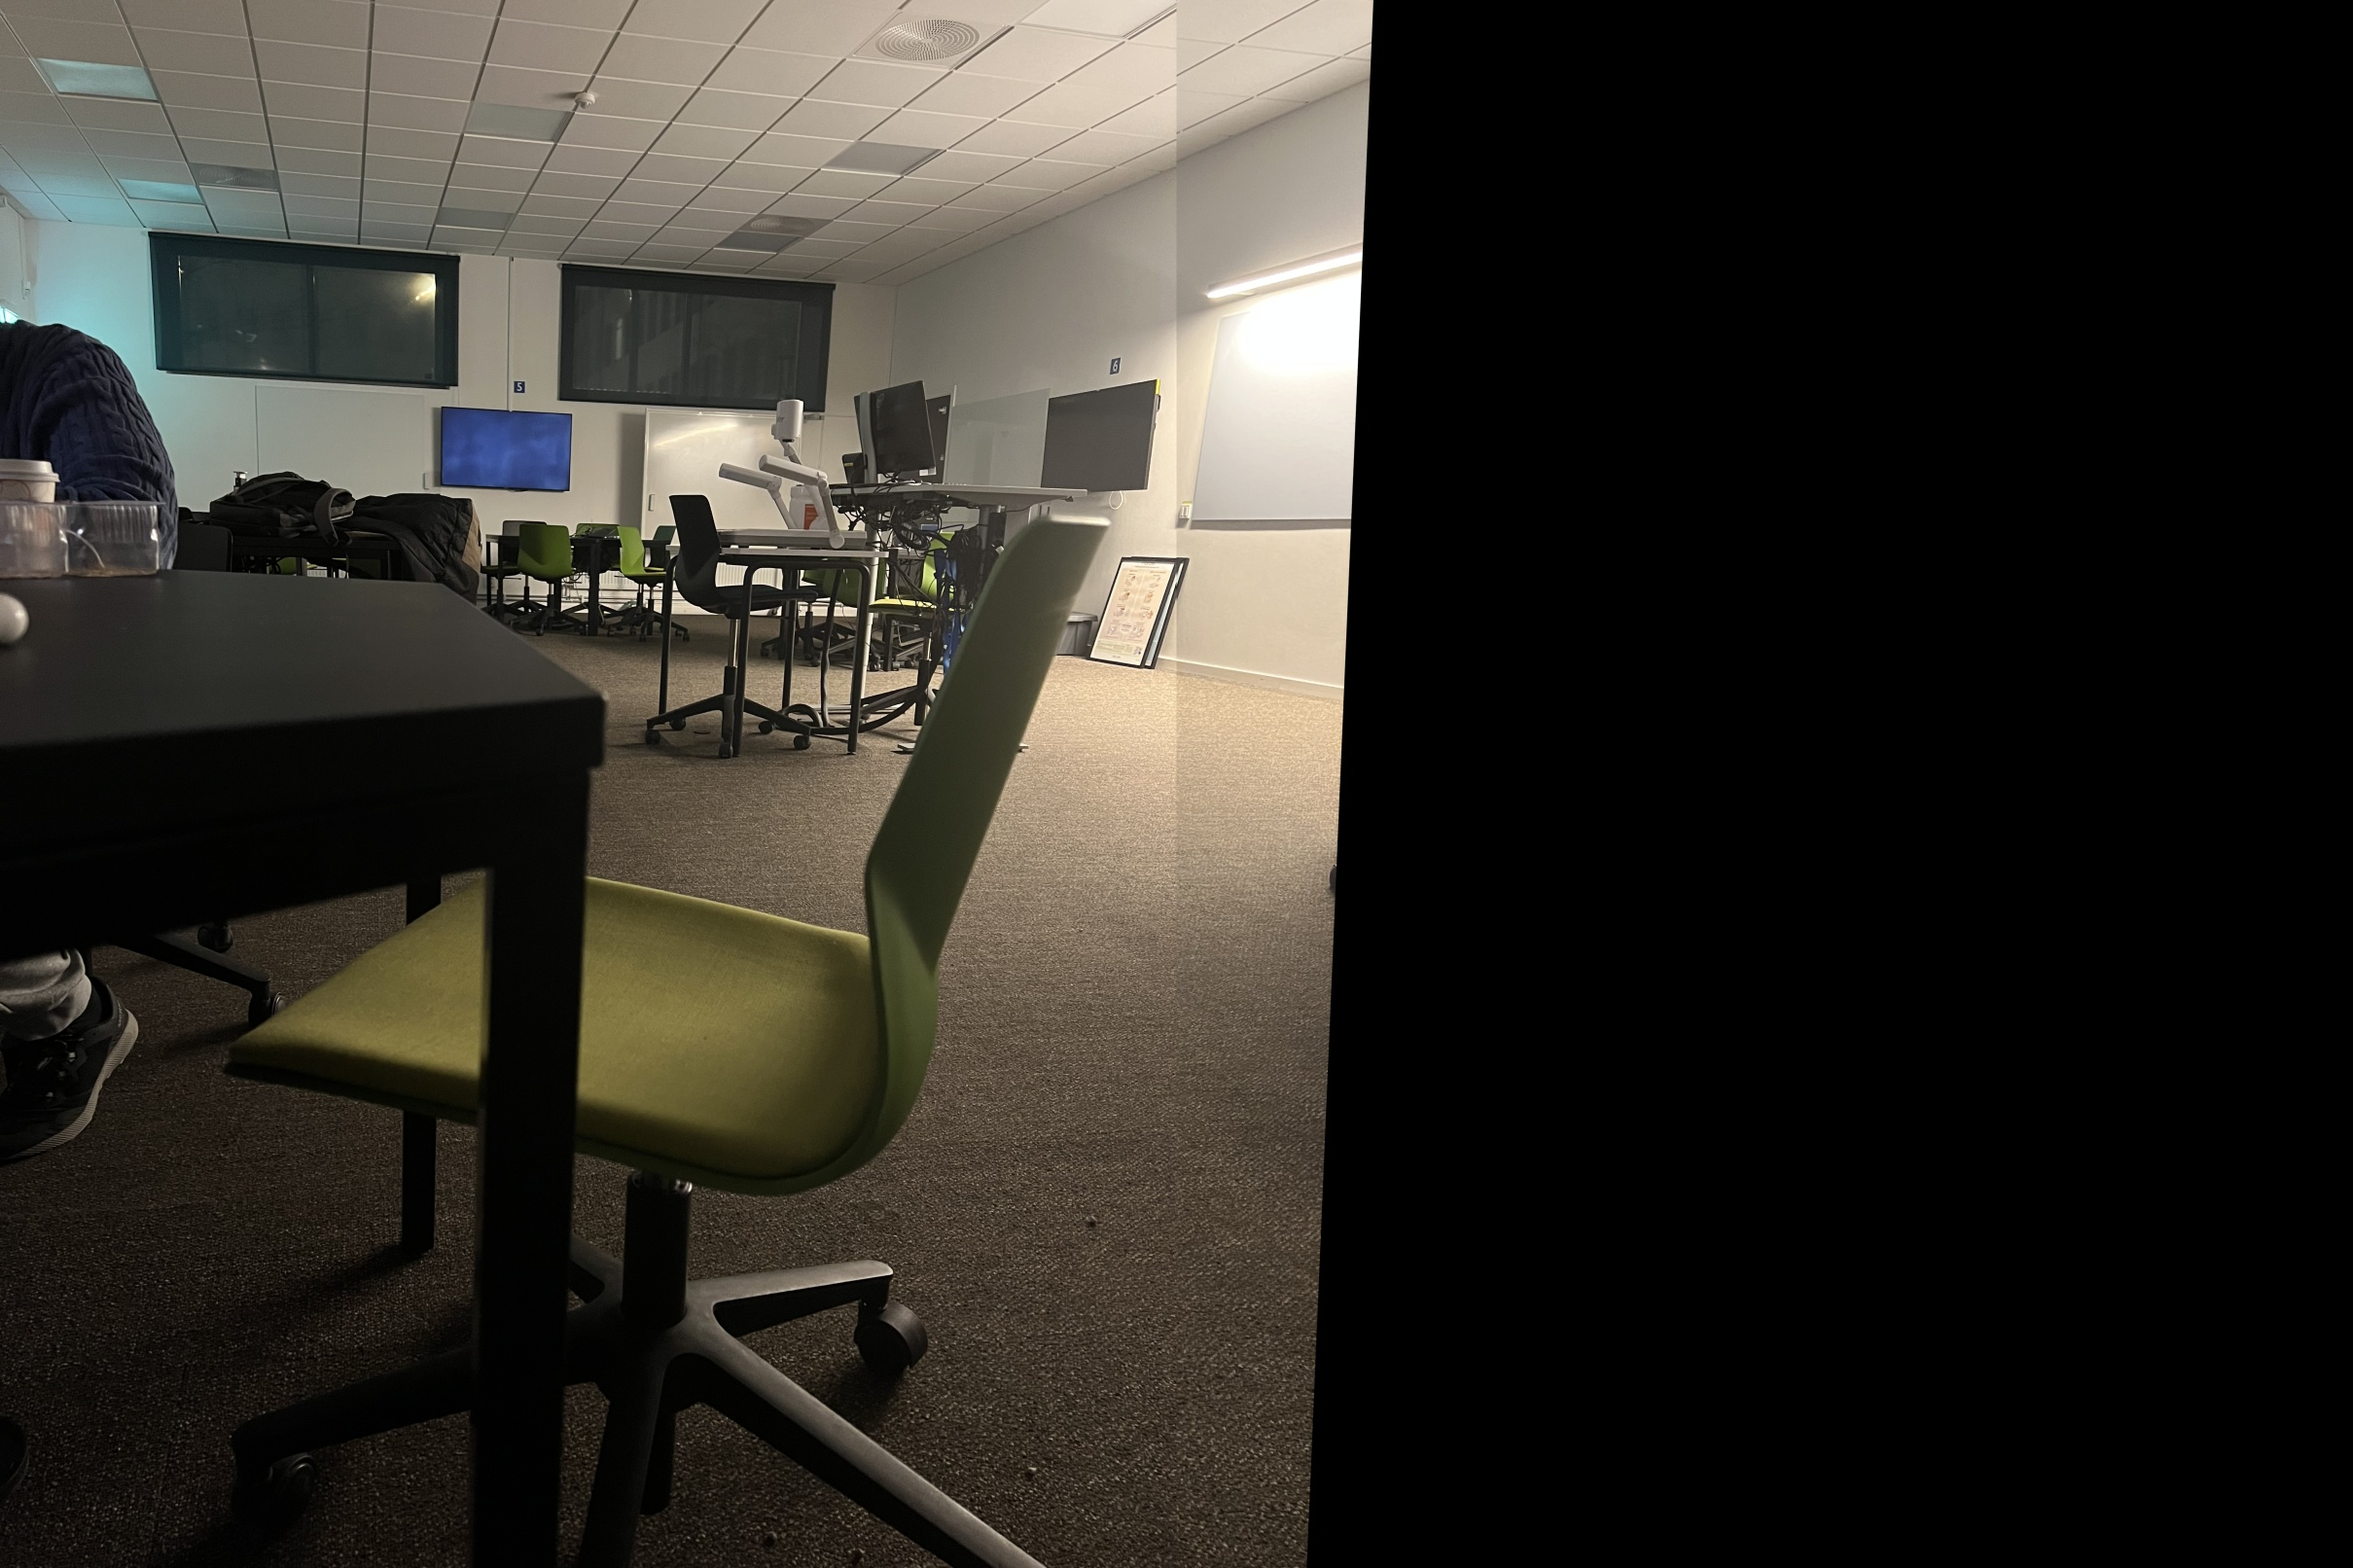
\includegraphics[width=1\textwidth]{output.jpg}
        \caption{Images produced image Stitching}
        \label{fig:stiched}
    \end{figure}

    \subsection{Reflection}
    This week was definitly the thoughest so far in regards to assingments. It took longer then I want to admit
    to grasp the concepts of homography matrices and how transfomrations work with images. It was hard to find good
    information on how Plane Sweep worked and it only became clear on how to implement it after the seminar. I started
    in the wrong end this week. The first thing I started with was image stitching. The implementation of this became 
    much easier when I fully understood how homography matrices works. It was really interesting to look at different
    methods for stereo matching.
    
    % Sources
    \newpage
    \printbibliography

    % Appendices
    \newpage
    \begin{appendices}
        \section{Python code for drawing Houh Transform}
        \label{appendix:hough}
        \begin{lstlisting}[language=python]
import matplotlib.pyplot as plt
import numpy as np

def getCrossLine(y1, y2, x):
    idx = np.argwhere(np.diff(np.sign(y1 - y2)) != 0)
    theta = x[idx]
    r = y1[idx]
    ixa = np.arange(start=0, stop=7, step=0.5)
    iya = np.zeros(len(ixa))
    for i in range(len(ixa)):
        iya[i] = ((-np.cos(theta)/np.sin(theta))*ixa[i]) + (r/np.sin(theta))
    return ixa, iya

thetas = np.deg2rad(np.arange(-90, 90))

xa = [2, 3, 6]
ya = [2, 1.5, 0]

ra = []
for i in range(len(xa)):
    temp = []
    for k in range(len(thetas)):
        temp.append(xa[i]*np.cos(thetas[k]) + ya[i] * np.sin(thetas[k]))
    ra.append(temp)


xc = [2, 5, 6]
yc = [2, 3, 0]
rc = []
for i in range(len(xc)):
    temp = []
    for k in range(len(thetas)):
        temp.append(xc[i]*np.cos(thetas[k]) + yc[i] * np.sin(thetas[k]))
    rc.append(temp)

ra = np.asarray(ra)
rc = np.asarray(rc)

ixa, iya = getCrossLine(ra[0], ra[1], thetas)

ixc1, iyc1 = getCrossLine(rc[0], rc[1], thetas)
ixc2, iyc2 = getCrossLine(rc[1], rc[2], thetas)
ixc3, iyc3 = getCrossLine(rc[0], rc[2], thetas)



fig , (ax1, ax2) = plt.subplots(1,2)
fig.suptitle('A')
ax1.scatter(xa, ya)
ax1.plot(ixa, iya)
for r in ra:
    ax2.plot(thetas, r)


fig2 , (cx1, cx2) = plt.subplots(1,2)
fig2.suptitle('C')
cx1.scatter(xc, yc)
cx1.plot(ixc1, iyc1)
cx1.plot(ixc2, iyc2)
cx1.plot(ixc3, iyc3)
for r in rc:
    cx2.plot(thetas, r)
plt.show()
        \end{lstlisting}

        \section{Harris implementation}
        \label{appendix:code}
        \begin{lstlisting}[language=Python]
import cv2
import numpy as np
import matplotlib.pyplot as plt


def harris(img_name, window_size, k, threshold):
    img = cv2.imread(img_name)
    gray = cv2.cvtColor(img, cv2.COLOR_BGR2GRAY)
    img_gauss = cv2.GaussianBlur(gray, (3, 3), 0)
    h = img.shape[0]
    w = img.shape[1]

    matrix_r = np.zeros((h, w))

    dx = cv2.Sobel(img_gauss, cv2.CV_64F,1,0, ksize=3)
    dy = cv2.Sobel(img_gauss, cv2.CV_64F, 0, 1, ksize=3)

    dx2 = np.square(dx)
    dy2 = np.square(dy)
    dxy = dx * dy

    offset = int(window_size/2)
    print("Finding corners...")
    for y in range(offset, h-offset):
        for x in range(offset, w-offset):
            sx2 = np.sum(dx2[y-offset:y+1+offset, x-offset:x+1+offset])
            sy2 = np.sum(dy2[y-offset:y+1+offset, x-offset:x+1+offset])
            sxy = np.sum(dxy[y-offset:y+1+offset, x-offset:x+1+offset])

            H = np.array([[sx2, sxy], [sxy, sy2]])
            det = np.linalg.det(H)
            tr = np.matrix.trace(H)
            R = det - k * (tr ** 2)
            matrix_r[y - offset, x - offset] = R

    cv2.normalize(matrix_r, matrix_r, 0, 1, cv2.NORM_MINMAX)
    for y in range(offset, h - offset):
        for x in range(offset, w - offset):
            value = matrix_r[y, x]
            if value > threshold:
                cv2.circle(img, (x, y), 3, (0, 255, 0))

    plt.figure("Harris detector")
    plt.imshow(cv2.cvtColor(img, cv2.COLOR_BGR2RGB)), plt.title("My Harris")
    plt.xticks([]), plt.yticks([])
    plt.show()

def cv2Harris(img_name):
    img = cv2.imread(img_name)
    gray = cv2.cvtColor(img, cv2.COLOR_BGR2GRAY)

    harris = cv2.cornerHarris(gray, 2, 3, 0.04)
    harris = cv2.dilate(harris, None)
    img[harris > 0.01 * harris.max()] = [0, 0, 255]

    plt.figure("Harris detector")
    plt.imshow(cv2.cvtColor(img, cv2.COLOR_BGR2RGB)), plt.title("CV2 Harris")
    plt.xticks([]), plt.yticks([])
    plt.show()

def cv2Sift(img_name):
    img = cv2.imread(img_name)
    gray = cv2.cvtColor(img, cv2.COLOR_BGR2GRAY)
    sift = cv2.SIFT_create()
    kp = sift.detect(gray, None)

    img = cv2.drawKeypoints(gray, kp, img)
    plt.figure("SIFT Detector")
    plt.imshow(img), plt.title("SIFT")
    plt.xticks([]), plt.yticks([])
    plt.show()

img_name = "start2.jpeg"

harris(img_name, 5, 0.04, 0.30)
cv2Harris(img_name)
cv2Sift(img_name)

        \end{lstlisting}
    \section{Python code for calculating the homography matrix}
    \label{appendix:homo}
    \begin{lstlisting}[language=Python]
import numpy as np

np.set_printoptions(suppress=True)

def calcHomo(p1, p2):
    A = []
    for i in range(0, len(p1)):
        x, y = p1[i][0], p1[i][1]
        u, v = p2[i][0], p2[i][1]
        A.append([x, y, 1, 0, 0, 0, -u*x, -u*y, -u])
        A.append([0, 0, 0, x, y, 1, -v*x, -v*y, -v])
    A = np.asarray(A)
    U, S, Vh = np.linalg.svd(A)
    L = Vh[-1,:] / Vh[-1,-1]
    H = L.reshape(3, 3)
    return H

def calcNewPoints(src, H):
    newPoints = []
    for x,y in src:
        vec = np.asarray([x,y,1])
        mult = H.dot(vec)
        newPoint = mult/mult[-1]
        newPoints.append([newPoint[0], newPoint[1]])

        
    return np.asarray(newPoints)

src = np.asarray([[0,0],[0,3],[5,3],[5,0]])
dst = np.asarray([[1,1],[3,3],[6,3],[5,2]])

H = calcHomo(src, dst)

print(H)

print(calcNewPoints(src, H))
        

    \end{lstlisting}
    \section{Python code for Plane Sweep}
    \label{appendix:PS}
    \begin{lstlisting}[language=python]
import cv2
import numpy as np

def depth(img1, img2, distance):
    height, width = img1.shape
    disparity = 0
    depthArray = np.zeros((height, width))
    maxDepth = 255/distance
    for y in range(0,height):
        for x in range(0, width):
            prev_min_val = np.inf
            for d in range(distance):
                temp_min_value = float(img1[y][x]) - float(img2[y][x-d])
                min_value = temp_min_value * temp_min_value
                if min_value < prev_min_val:
                    prev_min_val = min_value
                    disparity = d
            depthArray[y][x] = disparity * maxDepth
    cv2.imwrite("sd.png", depthArray)






img1 = cv2.imread("ps1.ppm", cv2.IMREAD_GRAYSCALE)
img2 = cv2.imread("ps2.ppm", cv2.IMREAD_GRAYSCALE)

stereo = cv2.StereoSGBM_create(numDisparities=16, blockSize=5)
disp = stereo.compute(img1,img2)
cv2.imwrite("cv2Sereo.png", disp)

depth(img1, img2, 16)
        
    \end{lstlisting}
    \section{Python code for Image Stitching}
    \label{appendix:IS}
        \begin{lstlisting}[language=python]
import cv2
import numpy as np
import random
np.set_printoptions(suppress=True)

def calcHomo(p1, p2):
    A = []
    for i in range(0, len(p1)):
        x, y = p1[i][0][0], p1[i][0][1]
        u, v = p2[i][0][0], p2[i][0][1]
        A.append([x, y, 1, 0, 0, 0, -u*x, -u*y, -u])
        A.append([0, 0, 0, x, y, 1, -v*x, -v*y, -v])
    A = np.asarray(A)
    U, S, Vh = np.linalg.svd(A)
    L = Vh[-1,:] / Vh[-1,-1]
    H = L.reshape(3, 3)
    return H

def geoDistance(p1, p2, h):
    p1 = p1[0]
    p2 = p2[0]
    p1 = np.append(p1, 1)
    p2 = np.append(p2, 1)
    estimatep2 = np.dot(h, p1)
    estimatep2 = estimatep2/estimatep2[-1]
    error = p2 - estimatep2

    return np.linalg.norm(error)


def ransac(src, dst, threshold):
    maxInliers = []
    finalH = None
    meme = 0
    for i in range(1000):
        meme = i
        p1 = []
        p2 = []
        #First cord:
        index = random.randrange(0, len(src))
        p1.append(src[index])
        p2.append(dst[index])
        #Second cord:
        index = random.randrange(0, len(src))
        p1.append(src[index])
        p2.append(dst[index])
        #Third cord:
        index = random.randrange(0, len(src))
        p1.append(src[index])
        p2.append(dst[index])
        #Fourth cord:
        index = random.randrange(0, len(src))
        p1.append(src[index])
        p2.append(dst[index])

        h = calcHomo(p1, p2)
        inlliers = []

        for i in range(len(src)):
            d = geoDistance(src[i], dst[i], h)
            if d<5:
                inlliers.append([src[i], dst[i]])
        
        if len(inlliers) > len(maxInliers):
            maxInliers = inlliers
            finalH = h
        if len(maxInliers) > (len(src) * threshold):
            break
    print("Num iter:",meme)
    return finalH



img1 = cv2.imread("right.jpg")
img2 = cv2.imread("left.jpg")

img1_gray = cv2.cvtColor(img1, cv2.COLOR_BGR2GRAY)
img2_gray = cv2.cvtColor(img2, cv2.COLOR_BGR2GRAY)

detector = cv2.ORB_create(nfeatures=2000)

keypoints1, descriptors1 = detector.detectAndCompute(img1, None)
keypoints2, descriptors2 = detector.detectAndCompute(img2, None)

bf = cv2.BFMatcher()
matches = bf.knnMatch(descriptors1,descriptors2, k=2)

# Ratio test
good_matches = []
for m, n in matches:
    if m.distance < 0.6 * n.distance:
        good_matches.append(m)


src_pts = np.float32([keypoints1[m.queryIdx].pt for m in good_matches]).reshape(-1, 1, 2)
dst_pts = np.float32([keypoints2[m.trainIdx].pt for m in good_matches]).reshape(-1, 1, 2)


H2, _ = cv2.findHomography(src_pts, dst_pts, cv2.RANSAC, 5.0)
H = ransac(src_pts, dst_pts, 0.74)

print(H)
print(H2)

result = cv2.warpPerspective(img1, H,(img1.shape[1] + img2.shape[1], img1.shape[0]))
result[0:img2.shape[0], 0:img2.shape[1]] = img2
cv2.imshow("Result", result)
result2 = cv2.warpPerspective(img1, H2,(img1.shape[1] + img2.shape[1], img1.shape[0]))

result2[0:img2.shape[0], 0:img2.shape[1]] = img2
cv2.imwrite("output.jpg", result)
cv2.waitKey()
        \end{lstlisting}
    \end{appendices}

\end{document}

% list with a,b,c
% \begin{enumerate}[label=(\alph*)]
%     \item 
% \end{enumerate}

% Centered figure with caption:
% \begin{figure}[H]
%     \centering
%     \includegraphics[width=1\textwidth]{%path} 
%     \caption{}
%     \label{fig:}
% \end{figure}

% Side by side figures:
% \begin{figure}[H]
%     \centering
%     \subfloat{{\includegraphics[width=0.46\textwidth]{%path} }}%
%     \qquad
%     \subfloat{{\includegraphics[width=0.46\textwidth]{%path} }}%
%     \caption{}
%     \label{fig:}
% \end{figure}

% Table with caption:
% \begin{table}[H]      
%     \begin{center}
%     \begin{tabular}{|c|c|} 
%         \hline
%         \textbf{} & \textbf{} \\\hline\hline
%          &  \\\hline 
%     \end{tabular}
%     \end{center}
%     \caption{}
%     \label{tab:}
% \end{table}

% Equation on multiple lines
% \begin{equation}
%    \begin{split}
%        x &= y \\
%        y &= z
%    \end{split}
% \end{equation}

% Code snippet
% \begin{lstlisting}%[language=]
%    //Code here
% \end{lstlisting}

% Code snippet from source file 
% \lstinputlisting[language=]{%path}
